% Problem 1 - Current amplifier design (15 points)
\Point{curramp}{minshortcircuitgain}{10}
\Point{curramp}{maxinputres}{2}
\Point{curramp}{equivalentvoltagegain}{3}
\begin{mainquestion}{curramp}{Current Amplifier Design}
The input of a current amplifier is to be connected to a current source with a source resistance $R_{s}$, and its output is connected to a load $R_{L}$, as shown below:

\begin{center}
\includegraphics[width=6in]{circuit.png}
\end{center}

You are to design the amplifier according to the following design constraints:

I. The attenuation loss at the amplifier input is at most 17\%.

II. Doubling $R_{L}$ should not change the output current by more than 17\%.

III. The overall current gain is at least 17.

\begin{partquestion}{minshortcircuitgain}{Find the minimum short-circuit current gain $A_{is}$.}
\begin{answer}
    \begin{kaitlyn}
    \noindent\fbox{%
\begin{minipage}{\dimexpr\textwidth-2\fboxsep-2\fboxrule\relax}
            \textbf{Why we're doing this problem:} Nothing is ever really $A_i i_i = i_o.$
            Why? Because the source and load attached to an amplifier (which is how any circuit exists) creates loading effects.
\end{minipage}%
      }%



The goal of this problem is to characterize the amplifier itself. Let's remember what an ideal current amplifier should do:

At the input for a current amplifier, we want as much of the source current as possible to enter the amplifier. Since the source current splits between $R_s$ and $R_i$, we want $R_i \rightarrow 0.$

At the output, the amplifier produces an output current that splits between $R_o$ and $R_L$. We want as much of that current as possible to enter the load, so we want $R_o \rightarrow \infty.$
Thus, an ideal current amplifier has $R_i = 0,$ and $R_o = \infty.$

However, as said in the question, the amplifier is connected to a source with a resistance and a load with its own resistance. These act as a voltage divider and create attenuation at the input and output and prevent our design from acting as the ideal current amplifier above, so we can find what fraction of the source current $i_s$ actually enters the input $i_i$:
\end{kaitlyn} 

    

\[
i_{i} = \frac{R_{s}}{R_{s} + R_{i}} i_{s}
\]

and

\[
i_{o} = \frac{R_{o}}{R_{o} + R_{L}} A_{is} i_{i}
\]

so

\[
A_{i} = \frac{i_{o}}{i_{s}} = \frac{R_{s}}{R_{s} + R_{i}} A_{is} \frac{R_{o}}{R_{o} + R_{L}}.
\]

The first term in this expression is input attenuation due to the current divider, and similarly, the last term is the output attenuation. To satisfy design constraint I, we require:

\begin{align*}
    \frac{R_s}{R_s + R_i} &\geq 0.83 \\
    0.17 R_s &\geq 0.83 R_i \\
    R_i &\leq 0.205R_s
\end{align*}

\begin{kaitlyn}

To satisfy constraint II, we can start from this:

\[i_o =\frac{R_o}{R_o+R_L}A_{is}i_i,\]

and say that increasing $R_L$ changes the output current division. If $R_L$ increases, less current is steered through the load and more remains through $R_o$, so $i_o$ decreases. We therefore compare the new output current with load $2R_L$ to the original output current with load $R_L$:

\[\frac{i_{o,2R_L}}{i_{o,R_L}} \geq 0.83.\]
    
\end{kaitlyn}

which can be simplified to:

\begin{align*}
    R_o + R_L &\geq 0.83R_o + 1.66R_L \\
    0.17 R_o &\geq 0.66 R_L \\
    R_o &\geq 3.88 R_L
\end{align*}

To ensure design constraint III (that the overall current gain meets the minimum value), we choose the worst-case values for the input and output resistances with $R_{i} = 0.205 R_{s}$ and $R_{o} = 3.88 R_{L}$. Plugging these into the expression for overall gain gives:

\begin{align*}
A_i &= \frac{R_s}{R_s + R_i} A_{is} \frac{R_o}{R_o + R_L} \geq 17 \\
&= \frac{R_s}{R_s + 0.205 R_s} A_{is} \frac{3.88 R_L}{3.88 R_L + R_L} \geq 17 \\
&= \frac{1}{1.205}A_{is} \frac{3.88}{4.88} \geq 17 \\
&= 0.660 A_{is} \geq 17
\end{align*}

and it follows that $A_{is,\min} = 25.7$.
\begin{kaitlyn}

\noindent\fbox{%
\begin{minipage}{\dimexpr\textwidth-2\fboxsep-2\fboxrule\relax}
        \textbf{Why this matters:} The amplifier itself must have a short-circuit current gain of at least $A_{is}=25.7$. Even though the desired \emph{overall} current gain is only 17, some of the available gain is lost because not all of the source current enters the amplifier and not all of the amplifier's output current reaches the load. The intrinsic amplifier must therefore provide extra gain to overcome these loading losses.
\end{minipage}%
}

\end{kaitlyn}
\end{answer}
\end{partquestion}

\begin{partquestion}{maxinputres}{If $R_{s} = 100\ \text{k}\Omega$ and $R_{L} = 1\ \text{k}\Omega$, find the maximum $R_{i}$ and the minimum $R_{o}$.}
\begin{answer}
From the results of part (\cref{prob:curramp:minshortcircuitgain}):

\[
R_{i} \leq 0.205 R_{s} = 0.205 \cdot 100\ \text{k}\Omega = 20.5\ \text{k}\Omega,
\]

and

\[
R_{o} \geq 3.88 R_{L} = 3.88 \cdot 1\ \text{k}\Omega = 3.88\ \text{k}\Omega.
\]
\end{answer}
\end{partquestion}

\begin{partquestion}{equivalentvoltagegain}{If this amplifier were to be represented by an equivalent voltage amplifier (with identical values for the three parameters found in parts (\cref{prob:curramp:minshortcircuitgain}) and (\cref{prob:curramp:maxinputres})), what would $A_{vo}$ be?}
\begin{answer}
Since the current amplifier would have an open-circuit output voltage of $A_{is} i_{i} R_{o}$, this must equal that of a standard voltage amplifier with open-circuit output voltage of $A_{vo} v_{i}$. Recall $i_{i} = \frac{v_{i}}{R_{i}}$ so we can write:

\begin{align*}
    A_{vo} v_i &= A_{is} i_{i} R_o \\
    A_{vo} v_i &= A_{is} \frac{v_i}{R_i} R_o \\
    A_{vo} &= A_{is} \frac{R_o}{R_i} \\
    &= 25.7 \frac{3.88}{20.5} \\
    &= 4.86
\end{align*}
\begin{kaitlyn}

\noindent\fbox{%
\begin{minipage}{\dimexpr\textwidth-2\fboxsep-2\fboxrule\relax}
        \textbf{Why this matters:} Remember ideals for a current amplifier:
        \begin{align*}
            R_i << R_s
        \end{align*} and
        \begin{align*}
            R_L << R_o
        \end{align*}

        because we want to design an easy path for all of the source current to enter the amplifier, rather than flow through the source's own impedance. \textbf{Once you connect amplifers to real devices, gain alone isn't the end of story -- we need to design its input and output impedances for the devices it interfaces with.}
\end{minipage}%
}

\end{kaitlyn}
\end{answer}
\end{partquestion}

\end{mainquestion}


% Problem 2 - Source follower measurement (10 points)
\clearpage
\Point{sourcefollower}{gm}{5}
\Point{sourcefollower}{ro}{5}
\begin{mainquestion}{sourcefollower}{Source Follower Measurement}

\begin{center}
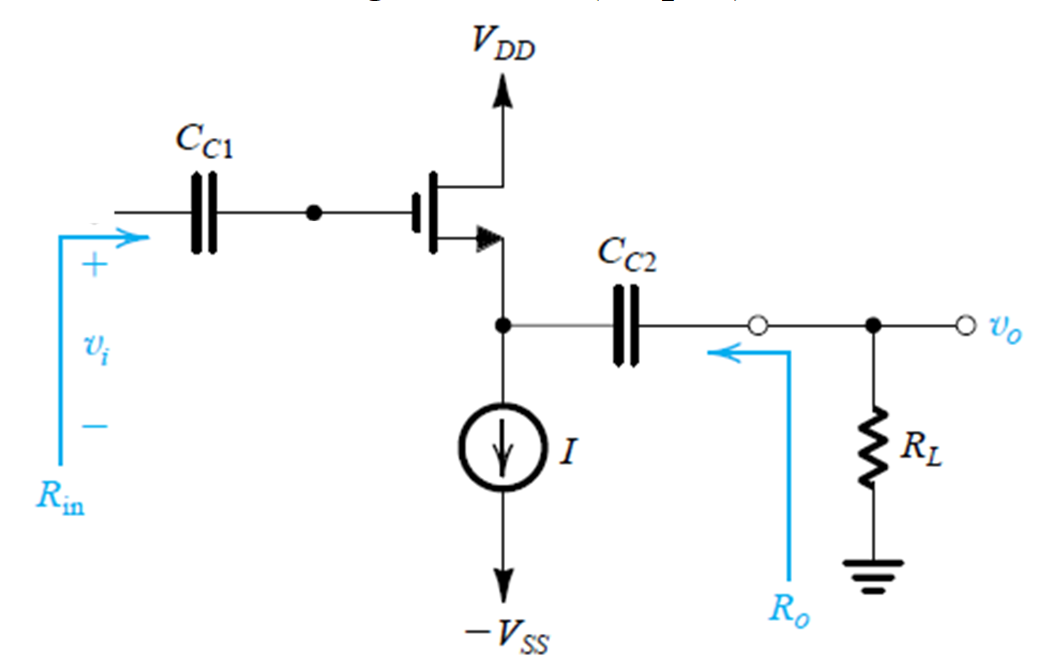
\includegraphics[width=4.5in]{questionbank/amplifiers/source_follower/v0/image7.png}
\end{center}

A source-follower circuit is shown below. With $R_L$ removed, the open-circuit voltage gain $A_{vo} = \frac{v_o}{v_i}$ is carefully measured and found to be 0.88. Then, when $R_L$  is connected and its value is varied, we find the gain is halved at $R_L = \qty{2}{\kilo\ohm}$. If the amplifier remained linear during the measurement, what are the values of $g_m$ and $r_o$?

\begin{partquestion}{gm}{Find $g_m$}
\begin{answer}

\begin{kaitlyn}
    \noindent\fbox{%
    \begin{minipage}{\dimexpr\textwidth-2\fboxsep-2\fboxrule\relax}   

        \textbf{How to approach this problem:} Use loading to determine the amplifier’s $R_o$, then zoom into the MOSFET small-signal model to determine what $g_m$ and $r_o$ produce that $R_o$

\end{minipage}%
}
\end{kaitlyn}
The open-circuit gain of the source follower (common-drain) stage without a load is:

\[
A_{vo} = \frac{v_{o}}{v_{i}} = \frac{g_{m} r_{o}}{1 + g_{m} r_{o}} = 0.88.
\]

With a load, the total gain is a voltage divider:

\[
A_{v} = A_{vo} \frac{R_{L}}{R_{L} + R_{o}}.
\]

If this gain is halved by connecting $R_{L} = \qty{2}{\kilo\ohm}$, then $R_{o} = \qty{2}{\kilo\ohm}$.

Since the resistance of the common drain output is $R_{o} = \frac{r_{o}}{1 + g_{m} r_{o}}$, taking the ratio of the first and third equations gives:

\[
g_{m} = \frac{A_{vo}}{R_{o}} = \frac{0.88}{2000} = 0.44\ \text{mS}.
\]
\end{answer}
\end{partquestion}

\begin{partquestion}{ro}{Find $\mathbf{r}_{\mathbf{o}}$}
\begin{answer}
Use the relationship between $R_{o}$, $g_{m}$, and $r_{o}$:

\[
R_{o} = \frac{r_{o}}{1 + g_{m} r_{o}} = \qty{2}{\kilo\ohm}.
\]

Solve for $r_{o}$ using the measured values:

\begin{align*}
    r_o &= \frac{R_o}{1 - R_o g_m} \\
    &= \frac{2000}{1 - 2000(0.00044)} = \qty{16.7}{\kilo\ohm}
\end{align*}

We can safely round this to \qty{17}{\kilo\ohm} to appease the universe. 

\end{answer}
\end{partquestion}

\end{mainquestion}


% Problem 3 - High-frequency pulse amplifier (13 points)
\clearpage
\Point{hfpulse}{amplifiertypes}{2}
\Point{hfpulse}{gm2}{2}
\Point{hfpulse}{currentpulse}{3}
\Point{hfpulse}{voltagepulse}{3}
\Point{hfpulse}{rdvalue}{3}
\begin{mainquestion}{hfpulse}{High-Frequency Pulse Amplifier}

The figure below shows a scheme for coupling and amplifying a high-frequency pulse signal. The circuit uses two MOSFETs whose details are not shown and a 50-$\Omega$ coaxial cable. For proper operation (with no signal reflections coming back down the cable), transistor $Q_{2}$ is required to present a 50-$\Omega$ resistance to the cable. That is, the input resistance for $Q_{2}$ is 50 $\Omega$.

\begin{center}
\includegraphics[width=4.5in]{pic6.png}
\end{center}

\begin{partquestion}{amplifiertypes}{In what type of amplifier is $Q_{1}$ operating? In what type of amplifier is $Q_{2}$ operating?}
\begin{answer}
$Q_{1}$ is a common source amplifier, with the input at the gate and the output at the drain. $Q_{2}$ is a common gate amplifier, with the input at the source and the output at the drain.
\end{answer}
\end{partquestion}

\begin{partquestion}{gm2}{What is $\mathbf{g}_{\mathbf{m2}}$?}
\begin{answer}
The input resistance to a common gate (CG) amplifier is $R_{\text{in}} = 1/g_{m} = 50\ \Omega$, so $g_{m2} = 0.02\ \text{S}$.
\end{answer}
\end{partquestion}

\begin{partquestion}{currentpulse}{If $Q_{1}$ and $Q_{2}$ are biased (operating) at the same point, what is the amplitude of the high-frequency current pulses in the drain of $Q_{1}$?}
\begin{answer}
Note that the current flowing through $Q_2$ all flows through $Q_1$. If the two transistors have the same current and the same overdrive voltage, then $g_{m1} = g_{m2} = 0.02\ \text{S}$. For an input amplitude of 3 mV, the output current amplitude is:

\[
0.003 \cdot 0.02 = 0.06\ \text{mA}.
\]

Note that because the CS is an inverting amplifier, the pulses will be negative.
\end{answer}
\end{partquestion}

\begin{partquestion}{voltagepulse}{What is the amplitude of the high-frequency voltage pulses at the drain of $Q_{1}$?}
\begin{answer}
Assuming $r_{o}$ is large enough to be ignored, the pulse amplitude is:

\[
g_{m} R v_{i} = (0.02)(50)(3\ \text{mV}) = 3\ \text{mV}.
\]

Again, the pulses will be negative due to the inverting amplifier.
\end{answer}
\end{partquestion}

\begin{partquestion}{rdvalue}{What is the value of $R_D$ required to provide 1-volt pulses at the drain of $Q_{2}$?}
\begin{answer}
The voltage gain of the CG amplifier is $g_{m}R_{D}$, and if we have 3 mV amplitude pulses at the input to $Q_2$ then (again when $r_{o}$ is sufficiently large) we have amplitude:

\begin{align*}
    R_D &= \frac{1}{g_m(0.003)} \\
    &= \frac{1}{(0.02)(0.003)} \\
    &= \qty{16.67}{\kilo\ohm}
\end{align*}

Shoot, we might as well just round up again to \qty{17}{\kilo\ohm}, since we are on a roll!

\end{answer}
\end{partquestion}

\end{mainquestion}


% Problem 4 - Cascaded CD and CG stages (14 points)
\clearpage
\Point{cascade}{cdgain}{5}
\Point{cascade}{cgopenocgain}{6}
\Point{cascade}{overallgain}{3}
\begin{mainquestion}{cascade}{Cascaded CD and CG Stages}

Consider cascading a common-drain and a common-gate stage, each of which has $g_m = 5\,\text{mS}$ and $r_o$ large enough to be ignored.

\begin{center}
\includegraphics[width=2.5in]{cd.png}\qquad
\includegraphics[width=2.5in]{cg.png}
\end{center}

\begin{partquestion}{cdgain}{Find the voltage gain $\frac{v_{o1}}{v_{i}}$ of the CD amplifier and its output resistance $R_{o1}$.}
\begin{answer}
The small signal model equivalent of this common drain stage is shown below:

\begin{center}
\includegraphics[width=2.5in]{sscd.png}
\end{center}

Neglecting channel length modulation ($r_o \rightarrow \infty$), the gain of the common-drain stage is:

\begin{align*}
v_{gs} &= v_i - v_{o1} \\
v_{o1} &= g_m v_{gs} R_s = g_m (v_i - v_{o1}) R_s \\
A_v &= \frac{v_{o1}}{v_i} = \frac{g_m R_S}{1 + g_m R_S} = \frac{(5)(3)}{1 + (5)(3)} = 0.9375
\end{align*}

We note this is the same form as in the lecture notes, but when $R_S$ is considered, it acts in parallel with $r_o$ , that is, ($r_o \parallel R_S$ ). However, because $r_o \rightarrow \infty$ , only $R_S$ remains, effectively taking the place of $r_o$.

The output resistance of the circuit can be found by shorting the input signal and applying a test source at the output terminals, as seen in the image below. The output resistance can be calculated by finding the current on the test voltage source.

\begin{center}
\includegraphics[width=2.5in]{rthcd.png}
\end{center}

We have:
\begin{align*}
    v_{gs} &= 0 - v_{x} \\
    i_{x} - \frac{v_{x}}{R_S} &= g_m v_{gs} = - g_m v_{x} \\
    R_{o1} &= \frac{v_{x}}{i_{x}} = \frac{R_S}{1+ g_m R_S} = \frac{3}{1 + (5)(3)} = \qty{0.188}{\kilo\ohm} = 188\Omega
\end{align*}

\end{answer}
\end{partquestion}

\begin{partquestion}{cgopenocgain}{Find the open-circuit voltage gain $\frac{v_{o}}{v_{i2}}$, the input resistance, and the output resistance of the CG amplifier.}
\begin{answer}

The small signal model equivalent of this common gate stage is shown below:

\begin{center}
\includegraphics[width=3.5in]{sscg1.png}
\end{center}

Neglecting channel length modulation, the gain of the common gate stage:

\begin{align*}
    v_{gs} &= 0 - v_{i2} \\
    v_o &= -(R_D \parallel R_L) g_m v_{gs} = (R_D \parallel R_L) g_m v_{i2}
\end{align*}

Recall we let $R_L \rightarrow \infty$ when considering open-circuit gain, so the circuit looks like:
\begin{center}
\includegraphics[width=3.5in]{sscg1b.png}
\end{center}
The gain is calculated as:
\begin{align*}
    A_{vo} &= \left.\frac{v_o}{v_{i2}}\right|_{R_L \rightarrow \infty} \\
    &= (R_D)g_m \\
    &= (20)(5) \\
    &= 100
\end{align*}


The input resistance can be found by calculating the current coming out of the input source:

\[
i_{i2}=\frac{v_{i2}}{R_{S}}-g_{m}v_{gs}=\frac{v_{i2}}{R_{S}}+g_{m}v_{i2} 
\]

And therefore:
\[
R_{i2}=\frac{v_{i2}}{i_{i2}}=\frac{1}{\frac{1}{R_{S}}+g_{m}}=\frac{1}{\frac{1}{10}+5}= \qty{0.196}{\kilo\ohm}=196\ \Omega
\]

The output resistance of the circuit can be found by shorting the input signal and applying a test source at the output terminals, as seen in the image below. 

\begin{center}
\includegraphics[width=4.5in]{sscg2.png}
\end{center}

From this circuit we can see that $v_{gs}=0$, so the dependent current source goes away.  Remember that we do not consider the load when calculating output resistance. It follows simply that:

\[ R_o = \qty{20}{\kilo\ohm}\]

\end{answer}
\end{partquestion}

\begin{partquestion}{overallgain}{Find the overall voltage gain $\frac{v_{o}}{v_{i}}$ if the output of the CD stage is connected to the input of the CG stage.}
\begin{answer}
The equivalent circuit of the cascaded amplifiers is shown below:

\begin{center}
\includegraphics[width=4.5in]{model.png}
\end{center}

We can write:
\begin{align*}
    G_v &= \frac{v_o}{v_i} \\
    &= (0.9375)\frac{R_{i2}}{R_{o1} + R_{i2}}(100)\left(\frac{R_L}{R_{o2} + R_L}\right) \\
    &= (0.9375)\frac{196}{196 + 188}(100)\left(\frac{11}{11 + 20}\right) \\
    &= 16.98 \approx 17
\end{align*}

\end{answer}
\end{partquestion}

\end{mainquestion}


% Problem 5 - Two-stage amplifier power analysis (18 points)
\clearpage
\Point{twostage}{stage1}{6}
\Point{twostage}{stage2}{6}
\Point{twostage}{overallgain}{3}
\Point{twostage}{power}{3}
\begin{mainquestion}{twostage}{Two-Stage Amplifier Power Analysis}

Consider the two-stage amplifier shown below. The coupling capacitors are "shorts" at the AC frequencies of interest. $V_t = 0.5\ \text{V}$ and $\lambda = 0.01\ \text{V}^{-1}$ for both transistors.

\begin{center}
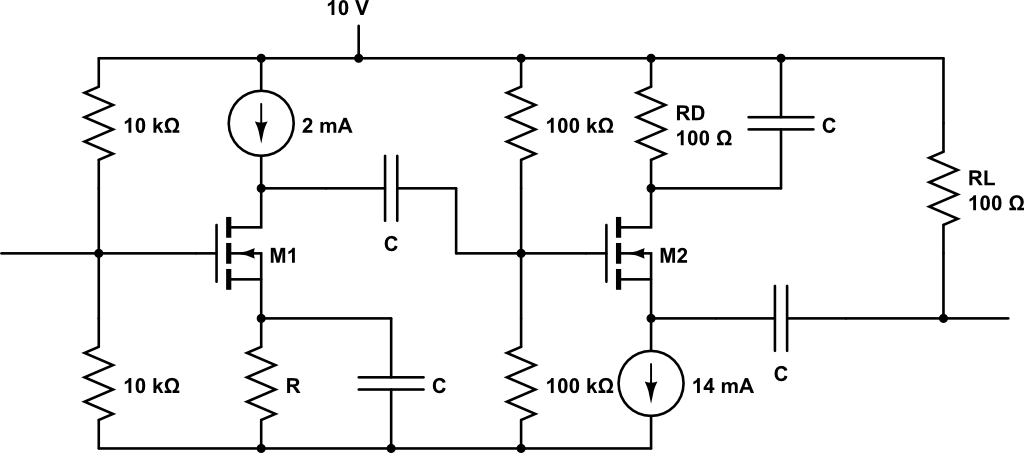
\includegraphics[width=4.5in]{questionbank/amplifiers/two_stage_power/v0/image87.png}
\end{center}

\begin{partquestion}{stage1}{What is Stage 1? Assume M1 is in saturation and evaluate the voltage gain $A_{v1}$, input resistance $R_{i1}$, and output resistance $R_{o1}$ given $k_{n1} = 1\ \frac{\text{mA}}{\text{V}^{2}}$.}
\begin{answer}

The first stage is delineated in the above drawing; it is a common source amplifier.  Note the input is at the gate and the output is taken from the drain.  It is clear that the current in M1 is $I_{D1}=2\text{\ mA}$.  It follows that:

\[
g_{m1} = \sqrt{2 k_{n1} I_{D1}} = \sqrt{2(1)(2)} = \qty{2}{\milli\siemens}
\]

and

\[
r_{o1} = \frac{1}{\lambda I_{D1}} = \frac{1}{(0.01)(2)} = \qty{50}{\kilo\ohm}
\]

The problem reminds us that the capacitors will become shorts in our frequency of interest. Therefore, the source resistor R is not part of the small signal analysis—it is only there to provide DC biasing.  Furthermore, the DC current source becomes an open circuit in small-signal analysis. These points help codify the small-signal equivalent circuit, which is shown below.

\begin{center}
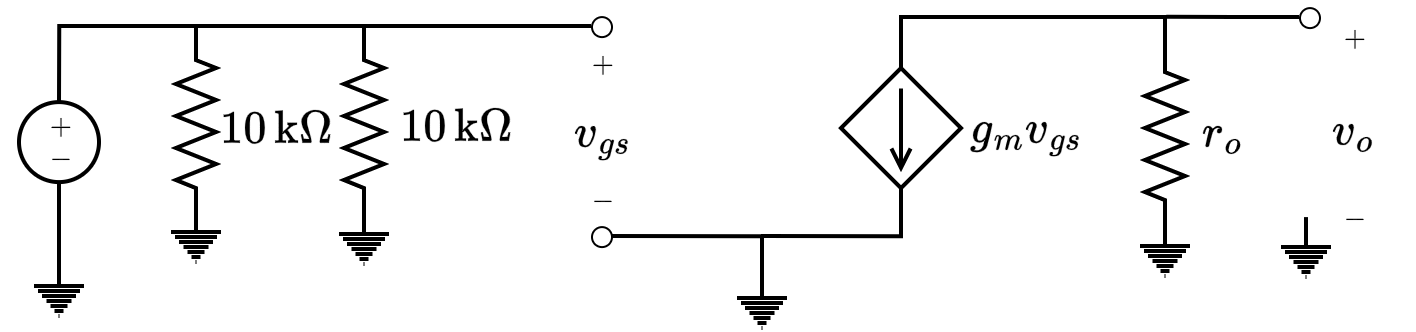
\includegraphics[width=4.5in]{questionbank/amplifiers/two_stage_power/v0/pic1.png}
\end{center}

The gain of this stage is given by:
\[ A_{v1} = -g_{m1}r_{o1} = -(2)(50) = -100\]
From the circuit above, we can find the input and output resistances:
\[R_{i1} = \qty{10}{\kilo\ohm} \parallel \qty{10}{\kilo\ohm} = \qty{5}{\kilo\ohm}\]
and
\[ R_{o1} = r_{o1} = \qty{50}{\kilo\ohm}\]
\end{answer}
\end{partquestion}

\begin{partquestion}{stage2}{What is Stage 2? Assume M2 is in saturation and evaluate the voltage gain $A_{v2}$, input resistance $R_{i2}$, and output resistance $R_{o2}$ given $k_{n2} = 3\ \frac{\text{mA}}{\text{V}^{2}}$.}
\begin{answer}
The second stage is delineated in the above drawing; it is a common drain amplifier.  Note the input is at the gate and the output is taken from the source.  It is clear that the current in M2 is $I_{D2}=14\text{\ mA}$.  It follows that:
\[
g_{m2} = \sqrt{2 k_{n2} I_{D2}} = \sqrt{2(3)(14)} =9.165\ \text{mS}
\]

and

\[
r_{o2} = \frac{1}{\lambda I_{D2}} = \frac{1}{(0.01)(14)} = 7.14\ \text{k}\Omega.
\]

For the AC analysis, the capacitor will be a short circuit in our frequency of interest, and the DC current source is an open circuit.  Our equivalent model is shown below:

\begin{center}
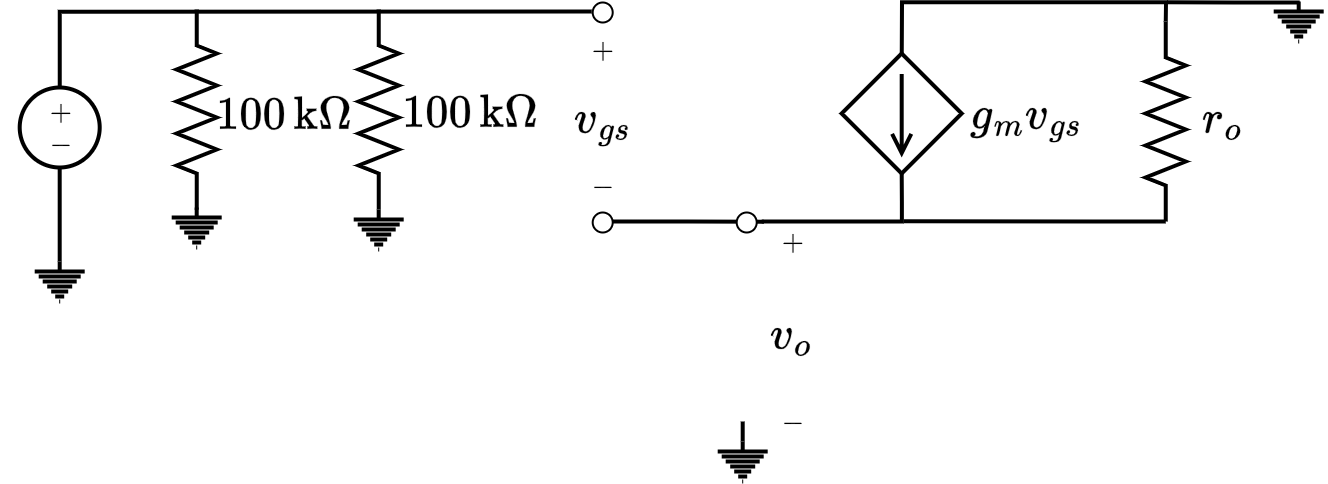
\includegraphics[width=4.5in]{questionbank/amplifiers/two_stage_power/v0/pic2.png}
\end{center}

To find the gain of this stage we have:
\begin{align*}
    v_{gs} &= v_i - v_o \\
    v_o &= g_{m2}v_{gs}r_{o2} = g_{m2}(v_i - v_o)r_{o2} \\
    v_o(1 + g_{m2}r_{o2}) &= g_{m2}r_{o2}v_i\\
\end{align*}

so, it follows that:

\[
A_{v2} = \frac{v_o}{v_i} = \frac{g_{m2}r_{o2}}{1 + g_{m2}r_{o2}} = \frac{(9.165)(7.14)}{1 + (9.165)(7.14)} = 0.985
\]

The input resistance is given by the two 100 kΩ resistors:
\[R_{i2}=100\text{\ k}\Omega \parallel 100\text{\ k}\Omega =50\text{\ k}\Omega \]

To find the output resistance, we short the input of the circuit and put a test source at the output, as shown below:

\begin{center}
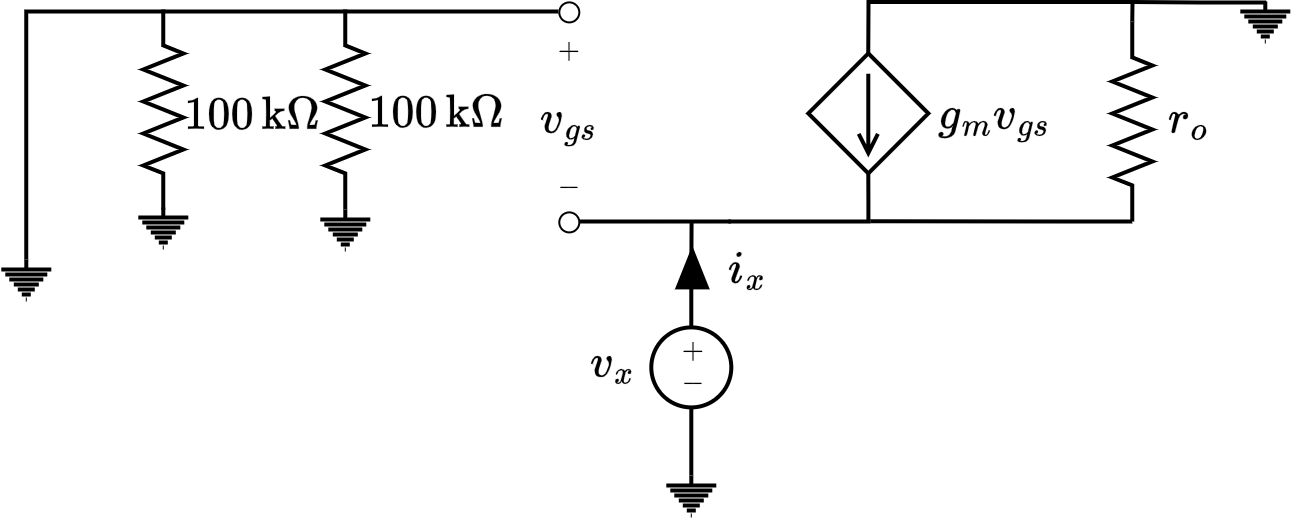
\includegraphics[width=4.5in]{questionbank/amplifiers/two_stage_power/v0/pic3.png}
\end{center}

We can calculate:

\begin{align*}
v_{gs}&=0-v_{x} \\
i_{x}+g_{m2}v_{gs}-\frac{v_{x}}{r_{o2}}&=0 \\
i_{x}-g_{m2}v_{x}-\frac{v_{x}}{r_{o2}}&=0
\end{align*}
so
\[
R_{o2}=\frac{v_{x}}{i_{x}}=\frac{r_{o2}}{1+g_{m}r_{o2}}=\frac{7.14}{1+\left(9.165\right)\left(7.14\right)}=107.47\ \Omega . 
\]
\end{answer}
\end{partquestion}

\begin{partquestion}{overallgain}{Find the overall voltage gain $\frac{v_{o}}{v_{i}}$.}
\begin{answer}

Drawing the equivalent circuit based on the results of the previous items:

\begin{center}
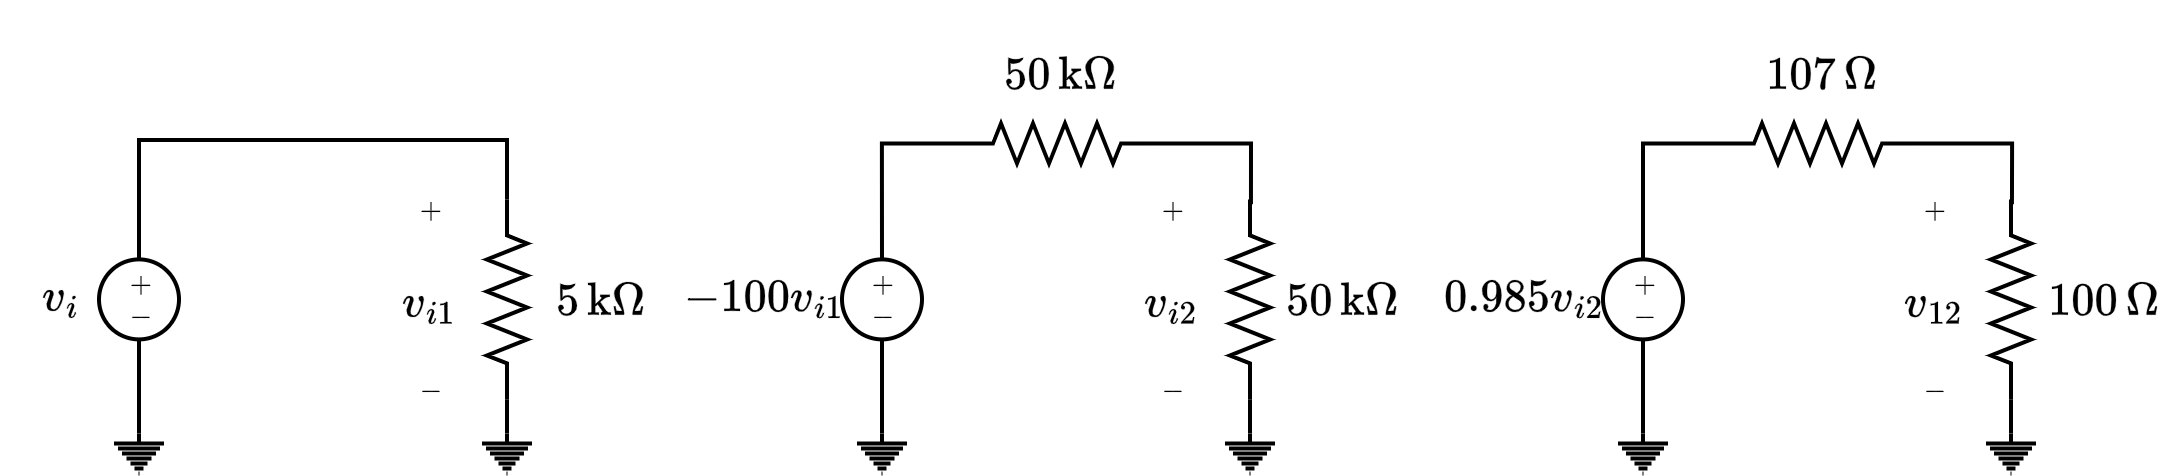
\includegraphics[width=6in]{questionbank/amplifiers/two_stage_power/v0/pic5.png}
\end{center}

We can calculate:
\begin{gather*}
    v_{i1}=v_{i} \\
    v_{i2}=-100v_{i1}\frac{50\text{\ k}\Omega }{50\text{\ k}\Omega +50\text{\ k}\Omega }=-50v_{i1} \\
    v_{o}=0.985v_{i2}\frac{100\ \Omega }{107.47\ \Omega +100\ \Omega }=0.4748v_{i_{2}}
\end{gather*}

So

\[
A_{v}=\frac{v_{o}}{v_{i}}=\left(0.4748\right)\left(-50\right)\left(1\right)=-23.74. 
\]
\end{answer}
\end{partquestion}

\begin{partquestion}{power}{Find the total DC power dissipated in the amplifier and the RMS power dissipated in the $100\,\Omega$ load if the input is $v_{i}(t) = 0.01 \sin \omega t$ V. What is the ratio between this RMS output power and the total DC power?}
\begin{answer}
The DC power dissipated in the amplifier is the sum of the power dissipated in each branch, including gate bias branches. We can use the fact that each branch drops the full 10 V input
across it:
\[P_{DC}=\left(2\text{\ mA\ +\ 14\ mA}\right)\left(10\text{\ V}\right)+\frac{{\left(10\text{\ V}\right)}^{2}}{20\text{\ k}\Omega }+\frac{{\left(10\text{\ V}\right)}^{2}}{200\text{\ k}\Omega }=165.5\text{\ mW.} \]
The RMS power dissipated in the load can be found using $v_{i}\left(t\right)$ and the total gain of the circuit:
\[P_{o,\text{RMS}}=\frac{{v_{o,\text{RMS}}}^{2}}{R_{L}}=\frac{{\left(A_{v}v_{i,\text{RMS}}\right)}^{2}}{R_{L}}=\frac{{\left(-23.74\frac{0.01}{\sqrt{2}}\right)}^{2}}{100\ \Omega }=0.282\text{\ mW.}\]
The small-signal output power is about:
\[\frac{0.282\text{\ mW}}{165.5\text{\ mW}}\times 100\%=0.17\% \]
of the total dissipated DC power.  Yee-haw!
\end{answer}
\end{partquestion}

\end{mainquestion}

